\documentclass{article}
\title{\LaTeX Math notes}
\author{Samuel Hautamäki}
\date{th of October 2024}
\usepackage{mathtools,amssymb,amsthm,gensymb,textcomp,graphicx}
\graphicspath{ {./} }
\begin{document}
  \maketitle
   
  \section{Degrees and radians}
  hl p 378\\
  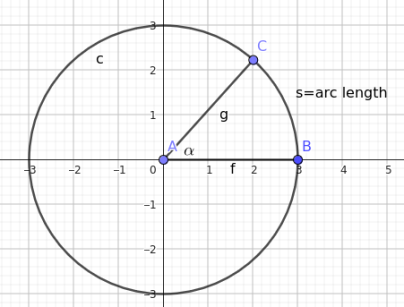
\includegraphics{arclength.png}
  substended angle $\alpha $has opposite arc with length s and radius R\\
  angle emasure as $radians=\alpha=\frac{s}{R}$\\
  Example\\
  a) $change 360\degree into radians$\\
  $\alpha=\frac{cirucmference of circle}{radius}=\frac{2\pi R}{R}=2\pi$\\ 
  so $360\degree=2\pi (radians)$\\
  b) Change $\pi$ radians into degrees.\\
  $360\degree=2\pi ||2$\\
  $180=\pi r$adians\\
  c) Change 3 radians into degrees\\
  $1\cdot\pi(radians)=180\degree ||:\pi$\\
  $1(radian)=\frac{180\degree}{\pi}$\\
  $3 radians =\frac{3\cdot180\degree}{\pi}$\\
  $3 radians= 172 (3.sf)$\\
  d) Change $1\degree$ into radians\\
  $180\degree=\pi$\\
  $1\degree=\frac{\pi}{180}$\\
  $1\degree=0.0175$ radians\\
  investigation 3 on hl p 379\\
  2. $2\pi$\\
  3. $360\degree=2\pi (radians)$\\
  360: $\frac{2\pi}{r}=2\pi$\\
  180: $\frac{\pi}{r}=\pi$\\
  90: $\frac{\pi}{2}$\\
  60: $\frac{\pi}{3}$\\
  45: $\frac{\pi}{4}$\\
  30: $\frac{\pi}{6}$\\
  4. A radian is a degree, but it's the length of the arc divided by radius. Can be expressed by pi.\\
  \subsection{excercises p 380}
  1. a. $45\degree=\frac{\pi}{4}$\\
  b. $\frac{\pi}{3}$\\
  c. $\pi+\frac{\pi}{2}$\\
  d. $2\pi$\\
  e. $\frac{\pi}{10}$\\
  f. $\pi+\frac{\pi}{4}$\\
  g. $4\cdot\frac{\pi}{9}$\\
  h. $\pi+\frac{\pi}{9}$\\
  i. $\frac{\pi}{2}+\frac{\pi}{6}$\\
  \subsection{revision of sectors}
  Area of sector=$\frac{\alpha}{360\degree}\cdot\pi R^2$\\
  In radians$\frac{1}{2}\cdot\beta\cdot R^2$\\
  Where $\alpha$ in degrees, and $\beta$ in radians.\\
  And length of arc $l=\frac{\alpha}{360\degree}\cdot2\pi R=\beta\cdot R$\\
  in formulabooklet!\\
  Ex. hl p383\\


   
\end{document}
